\section{Motivational Example}
\label{sec:example}
\begin{figure*}
  \subfloat[]
  {
    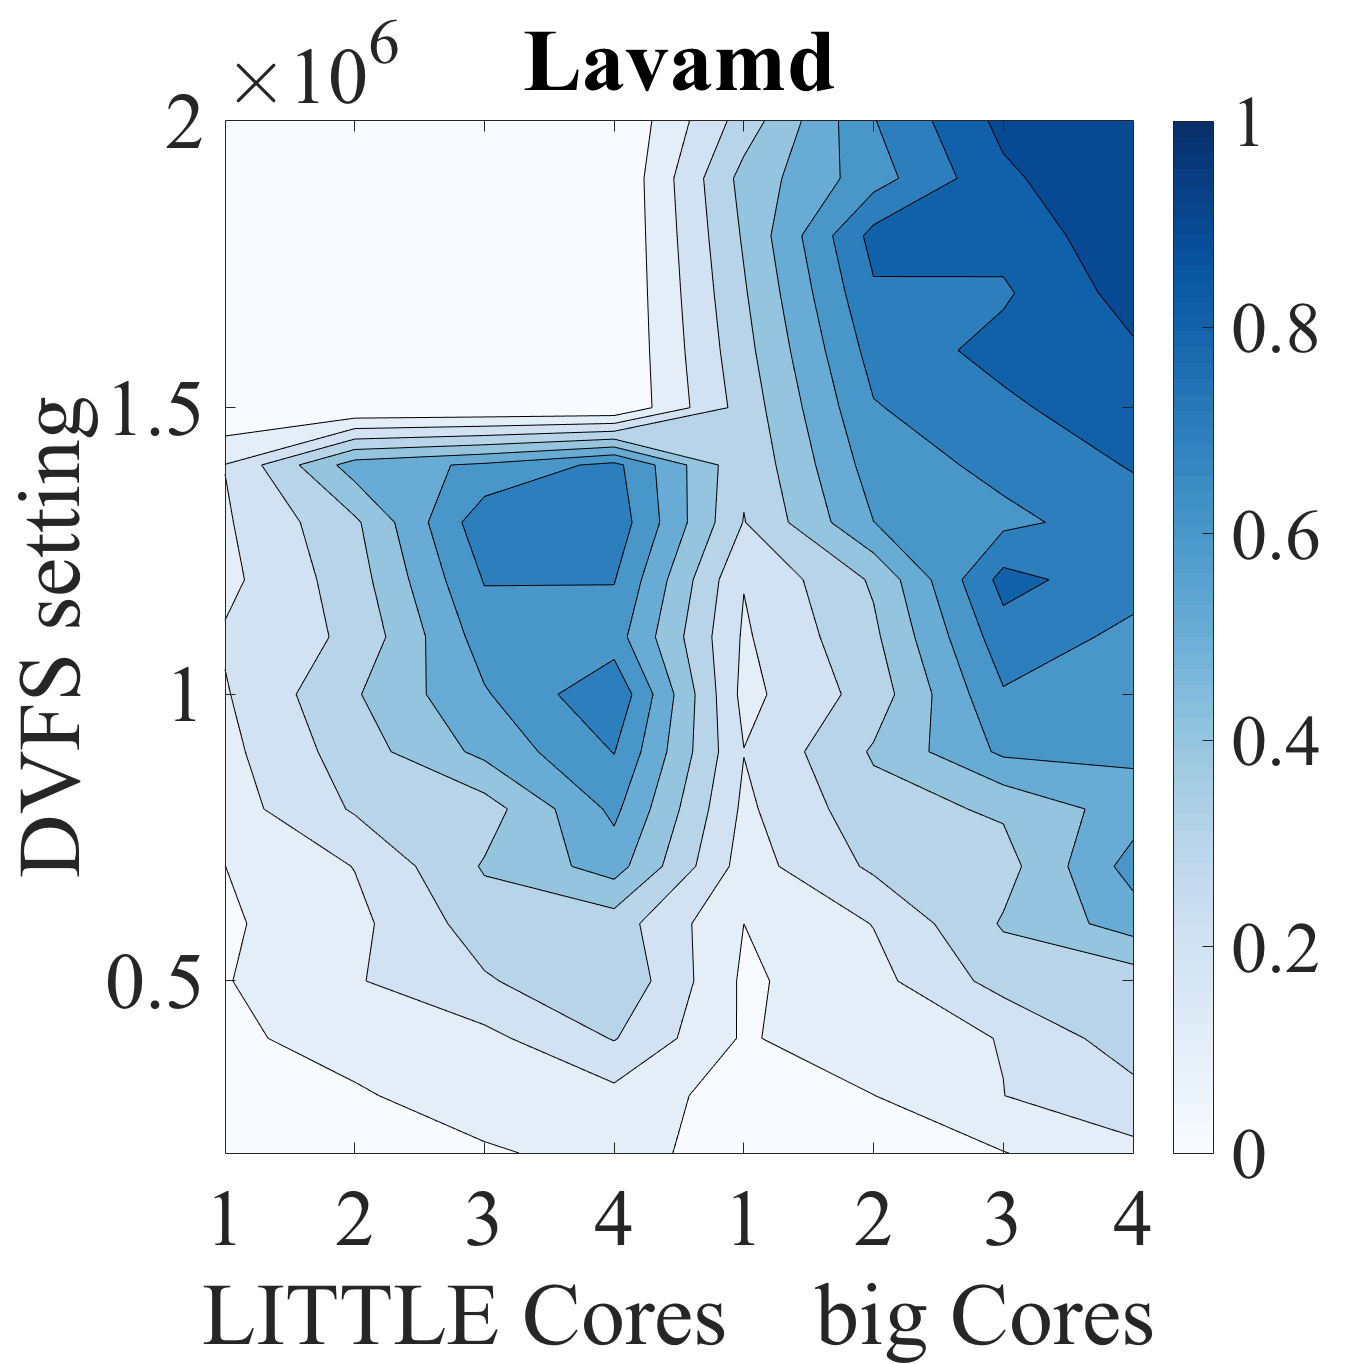
\includegraphics[width=.3\columnwidth]{figures/lavamd.png}
    \label{fig:lavamd_contour}
  }
  \subfloat[]
  {
    \begin{tikzpicture}
\begin{centering}

\begin{groupplot}[
    group style={
        group name=plots,
        group size=1 by 1,
        xlabels at=edge bottom,
        xticklabels at=edge bottom,
        vertical sep=5pt
    },
height=4.1cm,
width=0.45\columnwidth,
xmajorgrids,
ymajorgrids,
grid style={dashed},
xmax=20,
yticklabel pos=left,
enlargelimits=false,
tick align = outside,
tick style={white},
xticklabel shift={-5pt},
yticklabel shift={-5pt},
ylabel shift={-2pt},
ylabel style={align=center},
unbounded coords=jump,
]

\nextgroupplot[ylabel={\scriptsize Performance (Normalized)}, % Performance
xlabel={\footnotesize Iteration},
ytick={0.0,0.5,1.0,1.5,2.0},
yticklabels={,0.25,0.5,1.0,1.5},
legend entries={,{\scriptsize $\mathsf{Generic~Model}$},{\scriptsize $\mathsf{LAVAMD model}$}},
legend style={fill=none,draw=none,at={(0.5,1.4)},anchor=north,legend columns=1,line width=3pt},
]

\addplot[thick, dashed, black] coordinates {(10,0) (10,1.5)};
\addplot[thick, solid, color=poet] table[x index=0,y index=1,col sep=tab] {img/image_text/lavamd-example.txt};
\addplot[thick, solid, color=cal] table[x index=0,y index=2,col sep=tab] {img/image_text/lavamd-example.txt};
\end{groupplot}
\end{centering}
\end{tikzpicture}
    \label{fig:lavamd_timeline}
  }
  \caption{(a) Contour plot for normalized performance for \texttt{Lavamd} algorithm for different configurations(b) Time-line for running \texttt{Lavamd}. \emph{Control} is running in isolation without an HBM based \emph{learning} mechanism which leads to oscillations in the performance.}
  \label{fig:learning-models}
\end{figure*}

\begin{figure*}
  \subfloat[]
  {
    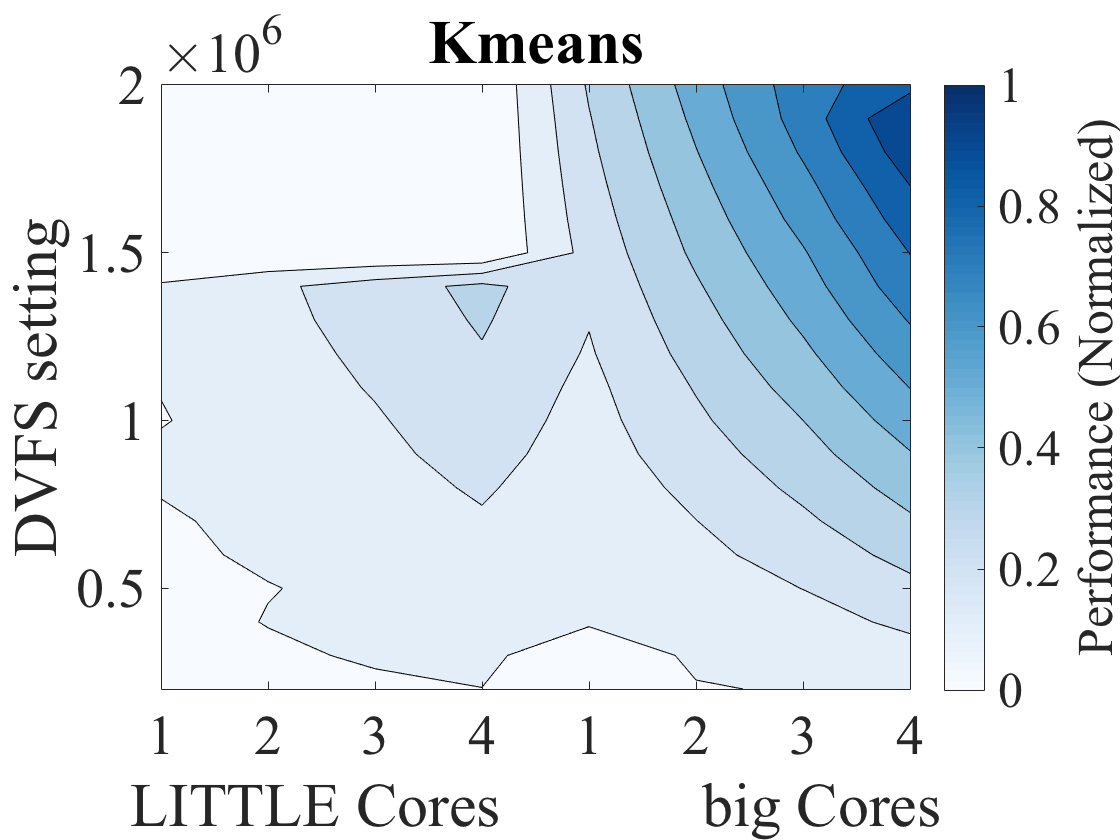
\includegraphics[width=.3\columnwidth]{figures/kmeans.png}
    \label{fig:kmeans_contour}
  }
  \subfloat[]
  {
    \begin{tikzpicture}
\begin{centering}

\definecolor{s1}{RGB}{228, 26, 28}
\definecolor{s2}{RGB}{55, 126, 184}
\definecolor{s3}{RGB}{77, 175, 74}
\definecolor{s4}{RGB}{152, 78, 163}
\definecolor{s5}{RGB}{255, 127, 0}

\begin{groupplot}[
    group style={
        group name=plots,
        group size=1 by 1,
        xlabels at=edge bottom,
        xticklabels at=edge bottom,
        vertical sep=5pt
    },
height=4cm,
width=1.3\columnwidth,
xmajorgrids,
ymajorgrids,
grid style={dashed},
xmin=0,
xmax=20,
yticklabel pos=left,
enlargelimits=false,
tick align = outside,
tick style={white},
xticklabel shift={-5pt},
yticklabel shift={-5pt},
ylabel shift={-2pt},
ylabel style={align=center},
unbounded coords=jump,
]

\nextgroupplot[ylabel={\footnotesize Performance \\ (Normalized)}, % Performance
%xtick={0,500,1000,1500,2000,2500,3000,3500,4000,4500},
ytick={0.0,0.5,1.0,1.5,2.0},
yticklabels={,0.5,1.0,1.5,2.0},
%xtick={0,30,60,120,160,200,240,280,320,480},
%xticklabels={,0,30,60,120,160,200,240,280,320,480},
%yticklabel style={font=\footnotesize},
xlabel={\footnotesize time (in sec)},
ymin=0,
ymax=1.5,
legend entries={,{$\mathsf{Learning}$},{$\mathsf{Control}$}},
legend style={draw=none,at={(0.5,1.3)},anchor=north,legend columns=4,
line width=5pt},
]

\addplot[thick, dashed, black] coordinates {(10,0) (10,1.5)};
\addplot[thick, solid, color=s4] table[x index=0,y index=1,col sep=tab] {img/image_text/kmeans-example.txt};
\addplot[thick, solid, color=s5] table[x index=0,y index=2,col sep=tab] {img/image_text/kmeans-example.txt};
%\addplot[thick, dashed, black] coordinates {(130,0) (130, 2)};
\end{groupplot}
\end{centering}

\end{tikzpicture}

    \label{fig:kmeans_timeline}    
  }
  \caption{(a) Contour plot for normalized performance for \texttt{Kmeans} algorithm for different configurations(b) Time-line for running \texttt{Kmeans} alone until 10 seconds, when another application. \emph{Learning} is running in isolation without an LCS based \emph{control} mechanism which leads to a performance drop which does not recover by itself.}
  \label{fig:learning-models}
\end{figure*}

We present two simple examples that illustrate the complementary
strengths and weaknesses of learning and control.  We use mobile
development boards featuring Samsung's Exynos 5 Octa with an ARM
big.LITTLE architecture that has four energy-efficient LITTLE cores
and four high-performance big cores.  Each core cluster can be set to
different clock speeds, leading to a large configuration space for
assigning resources to multi-threaded applications.

Each configuration (assignment of cores and clockspeeds) has different
performance, and this performance will be application dependent.
\figref{fig:lavamd_contour} and \figref{fig:kmeans_contour} show how
performance varies as a function of both resource usage and
application.  The figures show cores on the x-axis and clockspeed on
the y-axis, with performance shown as intensity -- darker colors
representing higher performance. The presence of local minima and
maxima mean that simple gradient ascent/descent methods are not
suitable to navigating these tradeoff spaces.
\figref{fig:lavamd_contour} and \figref{fig:kmeans_contour} also show
that the performance plot for the applications \texttt{lavamd} and
\texttt{kmeans} against the clockspeed and cores is non-convex and
contains at least 2 local minima corresponding to big and LITTLE
cores.  \texttt{lavamd} has other local minima and a significantly
more complicated tradeoff space than \texttt{kmeans}.

\PUNT{
\begin{figure}
\centering
%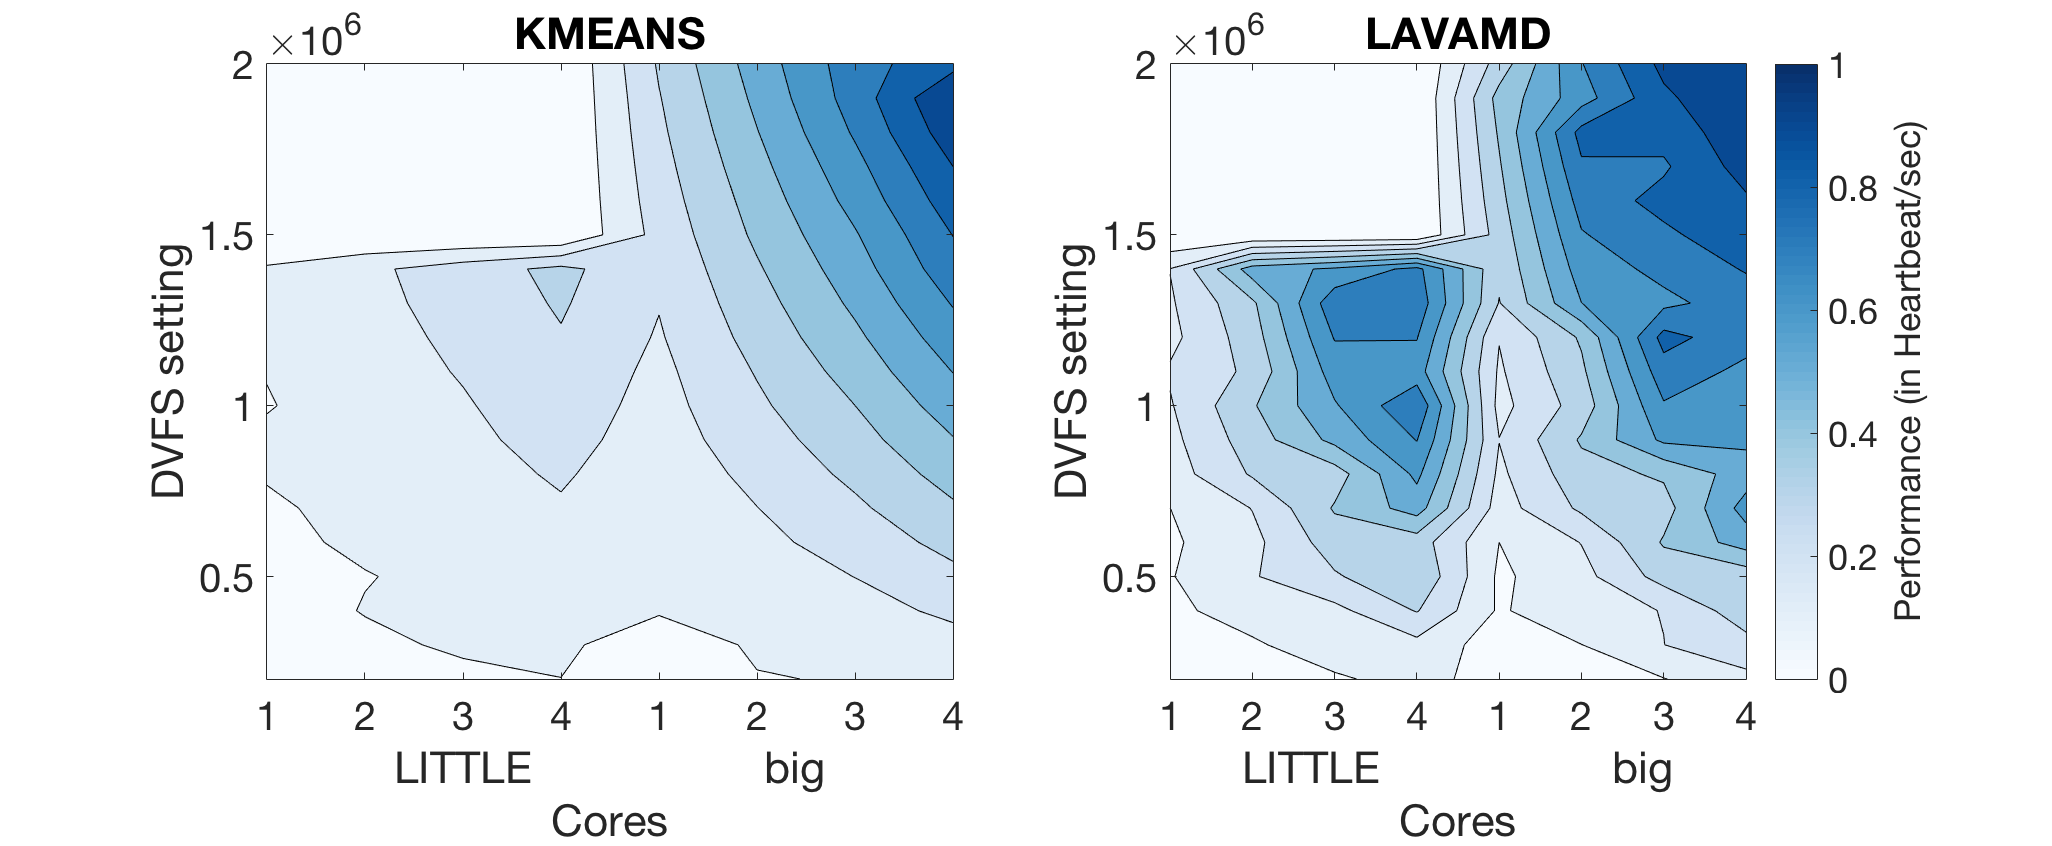
\includegraphics[width=\paperwidth,scale=0.5]{figures/performance-contour2.png}
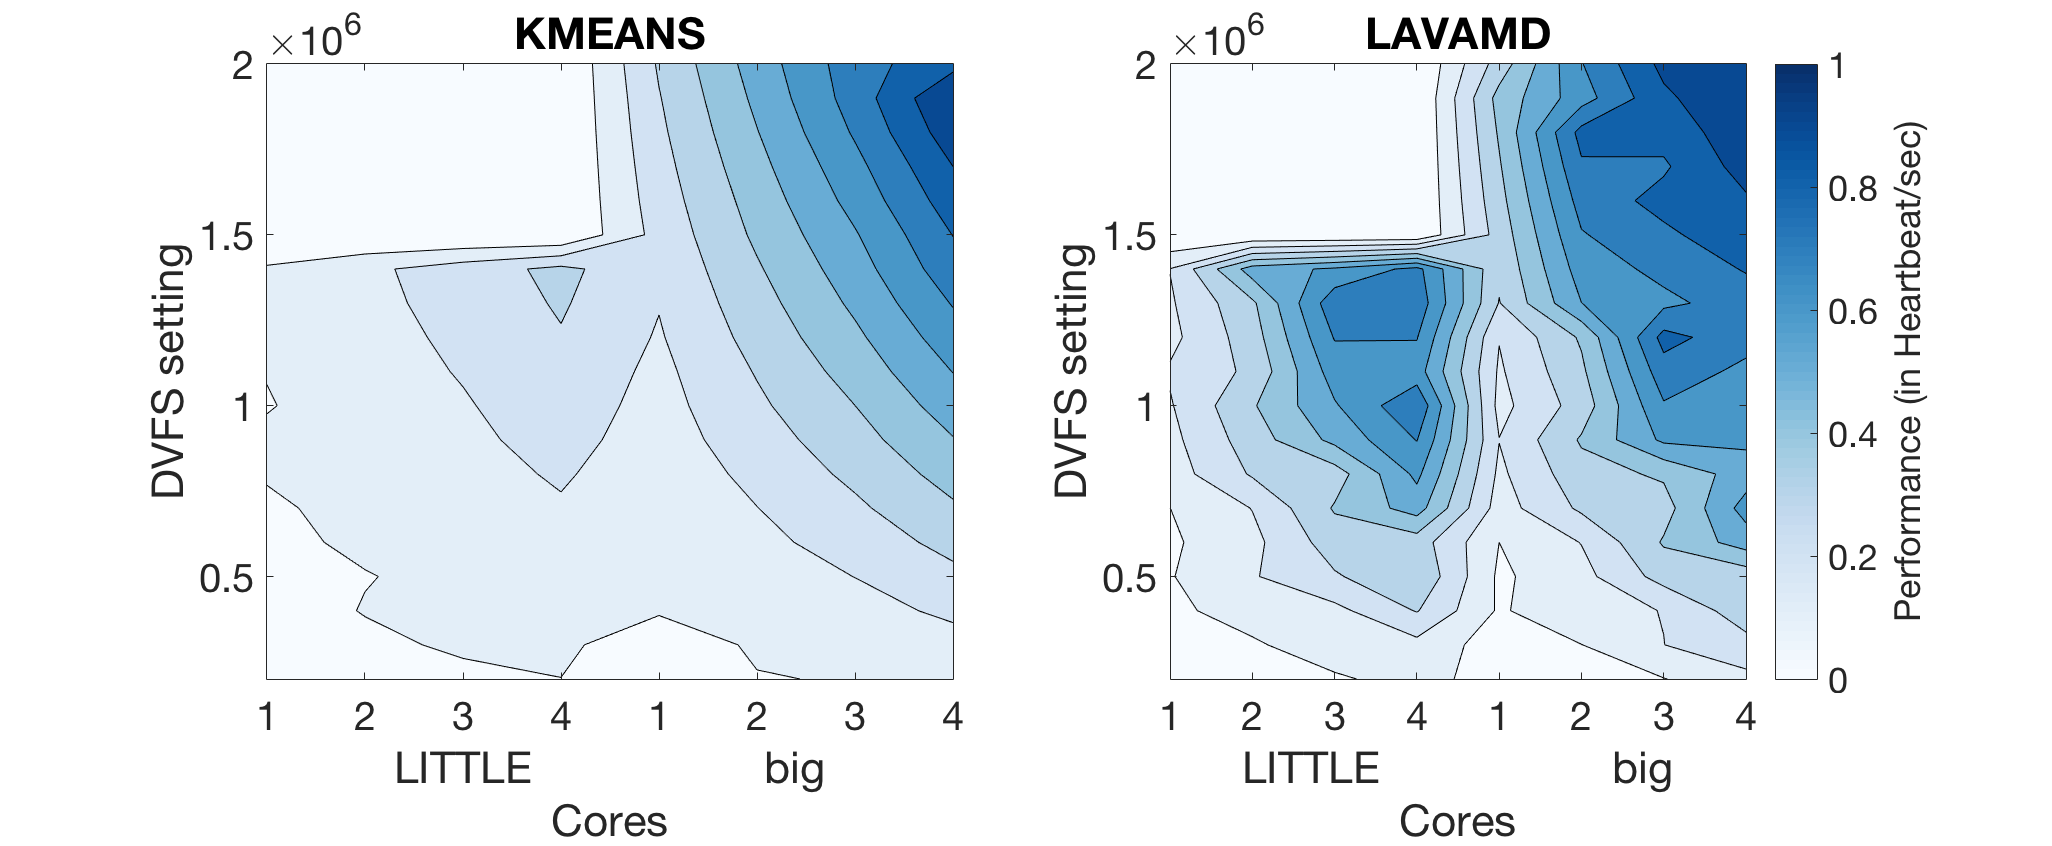
\includegraphics[width=\columnwidth]{figures/performance-contour2.png}
%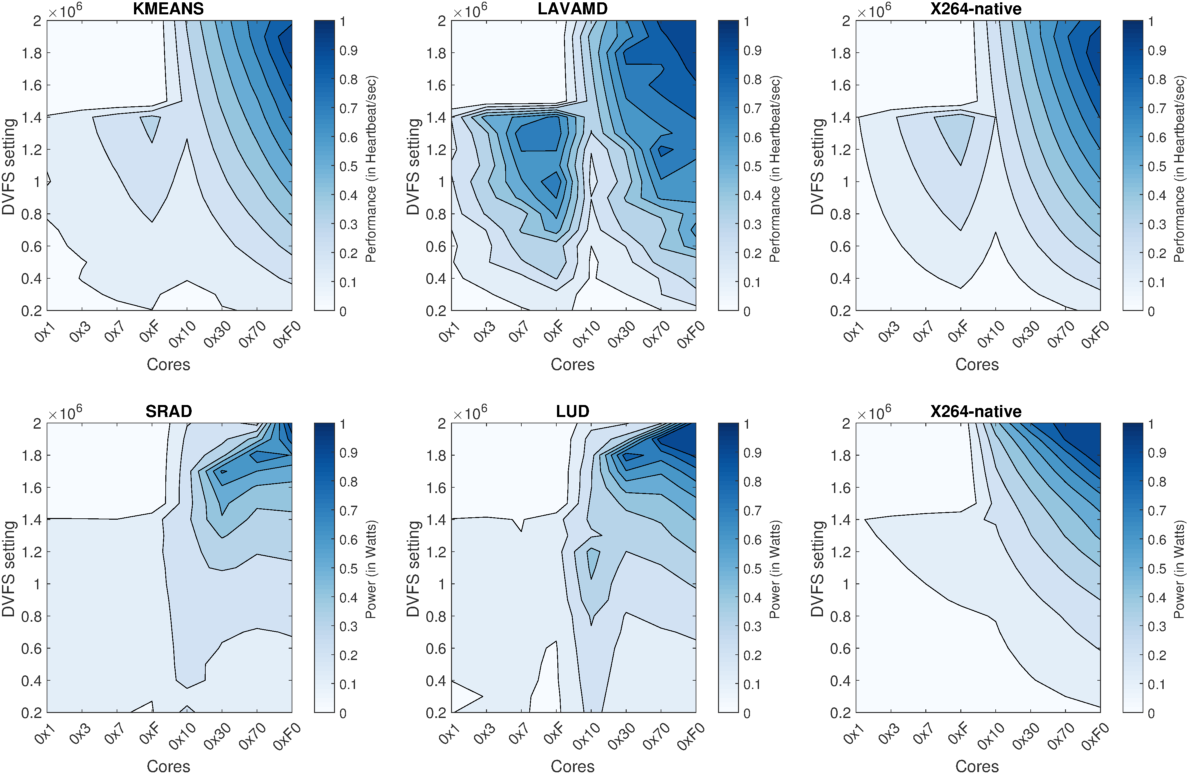
\includegraphics[scale=0.4]{figures/sample-contour3.png}
\caption{Contour plots showing performance as a function of core
  number, type, and speed.}
  \label{fig:contour}
\end{figure}
}

We consider prior \emph{learning} and \emph{control} approaches.  LEO,
a hierarchical Bayesian model based learner, estimates application
performance as a function of its resource usage \cite{LEO}. POET, a
control system, adjusts resource usage to meet application performance
requirements with minimal energy \cite{POET}.  We use this section to
develop intuition about the circumstances under which one performs
better than the other, motivating our proposal to combine the two.

\subsection{\emph{Learning} Complexity}
A number of machine learning approaches have been proposed to estimate
application performance in a variety of scenarios
\cite{reddiHPCA2013,LeeBrooks2006,CPR,ParallelismDial,Flicker,LeeBrooks,Koala}.
Machine learning is well suited to building models of complicated
systems like those shown in \figref{fig:lavamd_contour} and
\figref{fig:kmeans_contour} .

To demonstrate how well suited learning is to managing complexity, we
consider meeting a performance requirement for \texttt{lavamd}, the
application with a complicated configuration space.  We launch the
application with a soft performance constraint and both
\emph{learning} and \emph{control} adjust resource usage to meet that
requirement with minimal resource usage.  The \emph{learning} approach
estimates performance and power of all configurations and then uses
the lowest power configuration that meets the goal.  The
\emph{control} algorithm does not have a model of \texttt{lavamd}'s
complicated profile, but only has a knowledge of generic
power/performance frontiers (similar to \texttt{kmeans} in this
example) and it works by constantly measuring performance and
adjusting resource usage to see that goals are met.  While many
controllers use linear models, POET uses a convex model and handles
some non-linearities; however, it is sensitive to local maxima.
\PUNT{
\begin{figure}[t]
  \begin{tikzpicture}
\begin{centering}

\definecolor{s1}{RGB}{228, 26, 28}
\definecolor{s2}{RGB}{55, 126, 184}
\definecolor{s3}{RGB}{77, 175, 74}
\definecolor{s4}{RGB}{152, 78, 163}
\definecolor{s5}{RGB}{255, 127, 0}

\begin{groupplot}[
    group style={
        group name=plots,
        group size=1 by 1,
        xlabels at=edge bottom,
        xticklabels at=edge bottom,
        vertical sep=5pt
    },
height=3.5cm,
width=0.95\columnwidth,
xmajorgrids,
ymajorgrids,
grid style={dashed},
xmin=0,
xmax=29,
yticklabel pos=left,
enlargelimits=false,
tick align = outside,
tick style={white},
xticklabel shift={-5pt},
yticklabel shift={-5pt},
ylabel shift={-2pt},
ylabel style={align=center},
unbounded coords=jump,
]

\nextgroupplot[ylabel={\footnotesize Performance \\ (Normalized)}, % Performance
%xtick={0,500,1000,1500,2000,2500,3000,3500,4000,4500},
ytick={0.0,0.5,1.0,1.5,2.0},
yticklabels={,0.5,1.0,1.5,2.0},
%xtick={0,30,60,120,160,200,240,280,320,480},
%xticklabels={,0,30,60,120,160,200,240,280,320,480},
yticklabel style={font=\footnotesize},
ymin=0,
ymax=1.5,
legend entries={,{$\mathsf{Learning}$},{$\mathsf{Control}$}},
legend style={draw=none,at={(0.5,1.4)},anchor=north,legend columns=4,line width=5pt},
]

\addplot[thick, dashed, black] coordinates {(0,1) (29,1)};
\addplot[thick, solid, color=s4] table[x index=0,y index=2,col sep=tab] {img/image_text/lavamd-example.txt};
\addplot[thick, solid, color=s5] table[x index=0,y index=1,col sep=tab] {img/image_text/lavamd-example.txt};
%\addplot[thick, dashed, black] coordinates {(130,0) (130, 2)};
\end{groupplot}
\end{centering}

\end{tikzpicture}

   \vskip -1em
  \caption{Performance Control for LAVAMD}
  \label{fig:lavamd-example}
\end{figure}
} \figref{fig:lavamd_timeline} shows the results of controlling 30
iterations of \texttt{lavamd} to meet the performance requirement.
The x-axis shows iteration number and the y-axis shows performance
normalized to the
goal.  %There is a line for both LEO (labeled \emph{learning}) and POET (labeled \emph{control}).
In this case, the learning approach achieves the performance goal and
the controller oscillates wildly around it, sometimes not achieving
the goal and sometimes delivering performance that is too high (and
wastes energy). The problem stems from the fact that when the
performance goal is not met the learner would adjust the resources to
improve the performance based on an incorrect knowledge of the
performance trade-off space. Hence, the \emph{learner}'s ability to
handle complex models is crucial for reliable performance in this
example.

%This result may be somewhat counter-intuitive.  The problem is that the controller cannot handle the complexity of \texttt{lavamd}.  One way to fix this problem would be to build a custom controller just for this application, but that controller would not be useful for other applications.  In contrast, the learner can find the local maxima in the configuration space, and as this application has no phase changes or other dynamics, the one configuration that the learner finds is suitable for the entire application.

\subsection{\emph{Controlling} Dynamics}
We now consider controlling performance in a dynamic environment using
the \texttt{kmeans} application.  In this scenario, \texttt{kmeans}
begins as the only application running on the system.  Halfway through
its execution we launch a second application on a single big core.
This second application consumes about a quarter of the total
resources.  We again compare \emph{learning} and \emph{control}.

\PUNT{
\begin{figure}[t]
  \begin{tikzpicture}
\begin{centering}

\definecolor{s1}{RGB}{228, 26, 28}
\definecolor{s2}{RGB}{55, 126, 184}
\definecolor{s3}{RGB}{77, 175, 74}
\definecolor{s4}{RGB}{152, 78, 163}
\definecolor{s5}{RGB}{255, 127, 0}

\begin{groupplot}[
    group style={
        group name=plots,
        group size=1 by 1,
        xlabels at=edge bottom,
        xticklabels at=edge bottom,
        vertical sep=5pt
    },
height=3.5cm,
width=0.95\columnwidth,
xmajorgrids,
ymajorgrids,
grid style={dashed},
xmin=0,
xmax=20,
yticklabel pos=left,
enlargelimits=false,
tick align = outside,
tick style={white},
xticklabel shift={-5pt},
yticklabel shift={-5pt},
ylabel shift={-2pt},
ylabel style={align=center},
unbounded coords=jump,
]

\nextgroupplot[ylabel={\footnotesize Performance \\ (Normalized)}, % Performance
%xtick={0,500,1000,1500,2000,2500,3000,3500,4000,4500},
ytick={0.0,0.5,1.0,1.5,2.0},
yticklabels={,0.5,1.0,1.5,2.0},
%xtick={0,30,60,120,160,200,240,280,320,480},
%xticklabels={,0,30,60,120,160,200,240,280,320,480},
yticklabel style={font=\footnotesize},
ymin=0,
ymax=1.5,
legend entries={,{$\mathsf{Learning}$},{$\mathsf{Control}$}},
legend style={draw=none,at={(0.5,1.4)},anchor=north,legend columns=4,line width=5pt},
]

\addplot[thick, dashed, black] coordinates {(10,0) (10,1.5)};
\addplot[thick, solid, color=s4] table[x index=0,y index=1,col sep=tab] {img/image_text/kmeans-example.txt};
\addplot[thick, solid, color=s5] table[x index=0,y index=2,col sep=tab] {img/image_text/kmeans-example.txt};
%\addplot[thick, dashed, black] coordinates {(130,0) (130, 2)};
\end{groupplot}
\end{centering}

\end{tikzpicture}

   \vskip -1em
  \caption{Performance Control for KMEANS}
  \label{fig:kmeans-example}
\end{figure}
}

\figref{fig:kmeans_timeline} shows the results of this experiment,
with time on the x-axis and performance on the y-axis, normalized to
the target.  The vertical dashed line shows when the second
application begins.  The figure clearly shows the benefits of a
control system in this scenario.  After a small dip in performance,
the controller adjusts to return it back to the desired level.  The
learning system however, does not have any inherent mechanism to
measure the change or adapt to the altered performance.  While we
could theoretically relearn the tradeoff space every time the
environment changes, doing so is impractical.

Control systems are a great light-weight mechanisms for managing such
dynamics. The control systems provide the necessary robustness to a
system prone to such dynamics and fluctuations
\cite{Hellerstein2004a}. Control systems are resilient to scale change
in the system performance or power, and many dynamic changes reduce
the performance of all configurations uniformly, affecting the scale
of the performance but keeping the shape of the space intact.  For
this reason, control systems have been widely used to manage computing
systems that have to deal with dynamic fluctuations.  These approaches
have been especially successful in webservers with fluctuating request
rates \cite{Horvarth,LuEtAl-2006a,SunDaiPan-2008a} and multimedia
applications which have to deal with multiple phases with different
resource demands \cite{TCST,Agilos,grace2}.

\PUNT{ The primary contribution of this paper is to combine a learning
  technique that can handle complexity with a control system that can
  handle dynamic environments.  }

%%
\PUNT{
\begin{figure}
\centering
%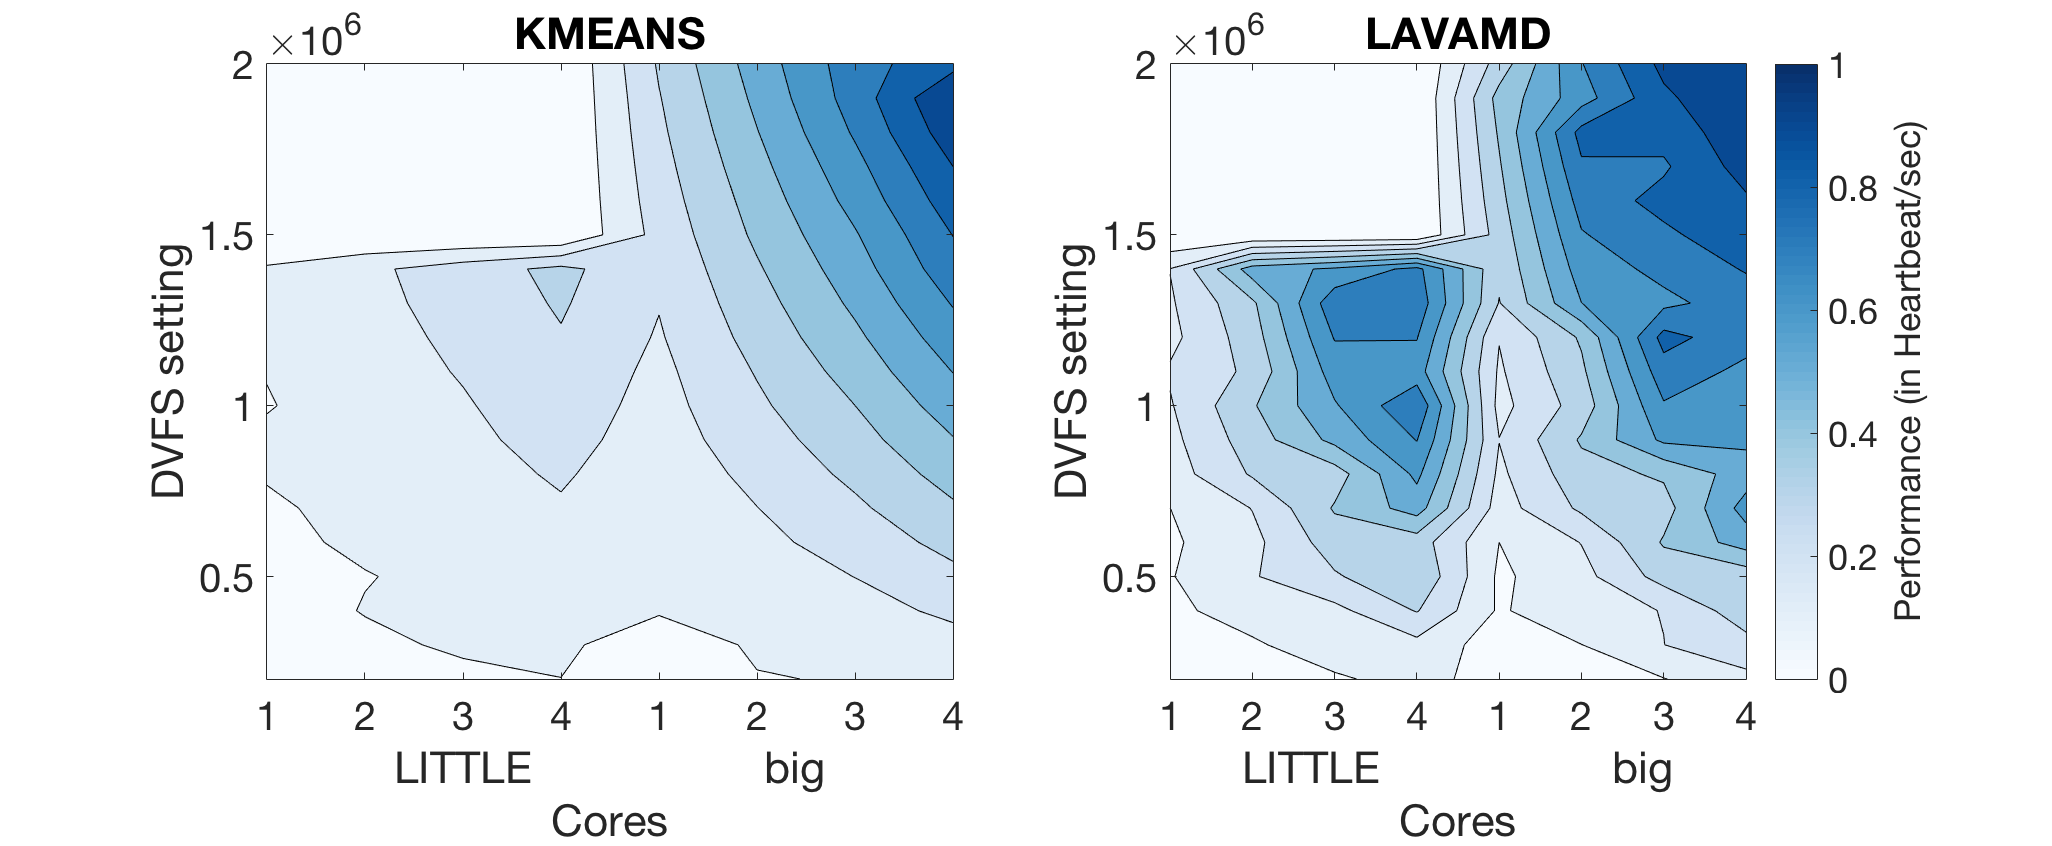
\includegraphics[width=\paperwidth,scale=0.5]{figures/performance-contour2.png}
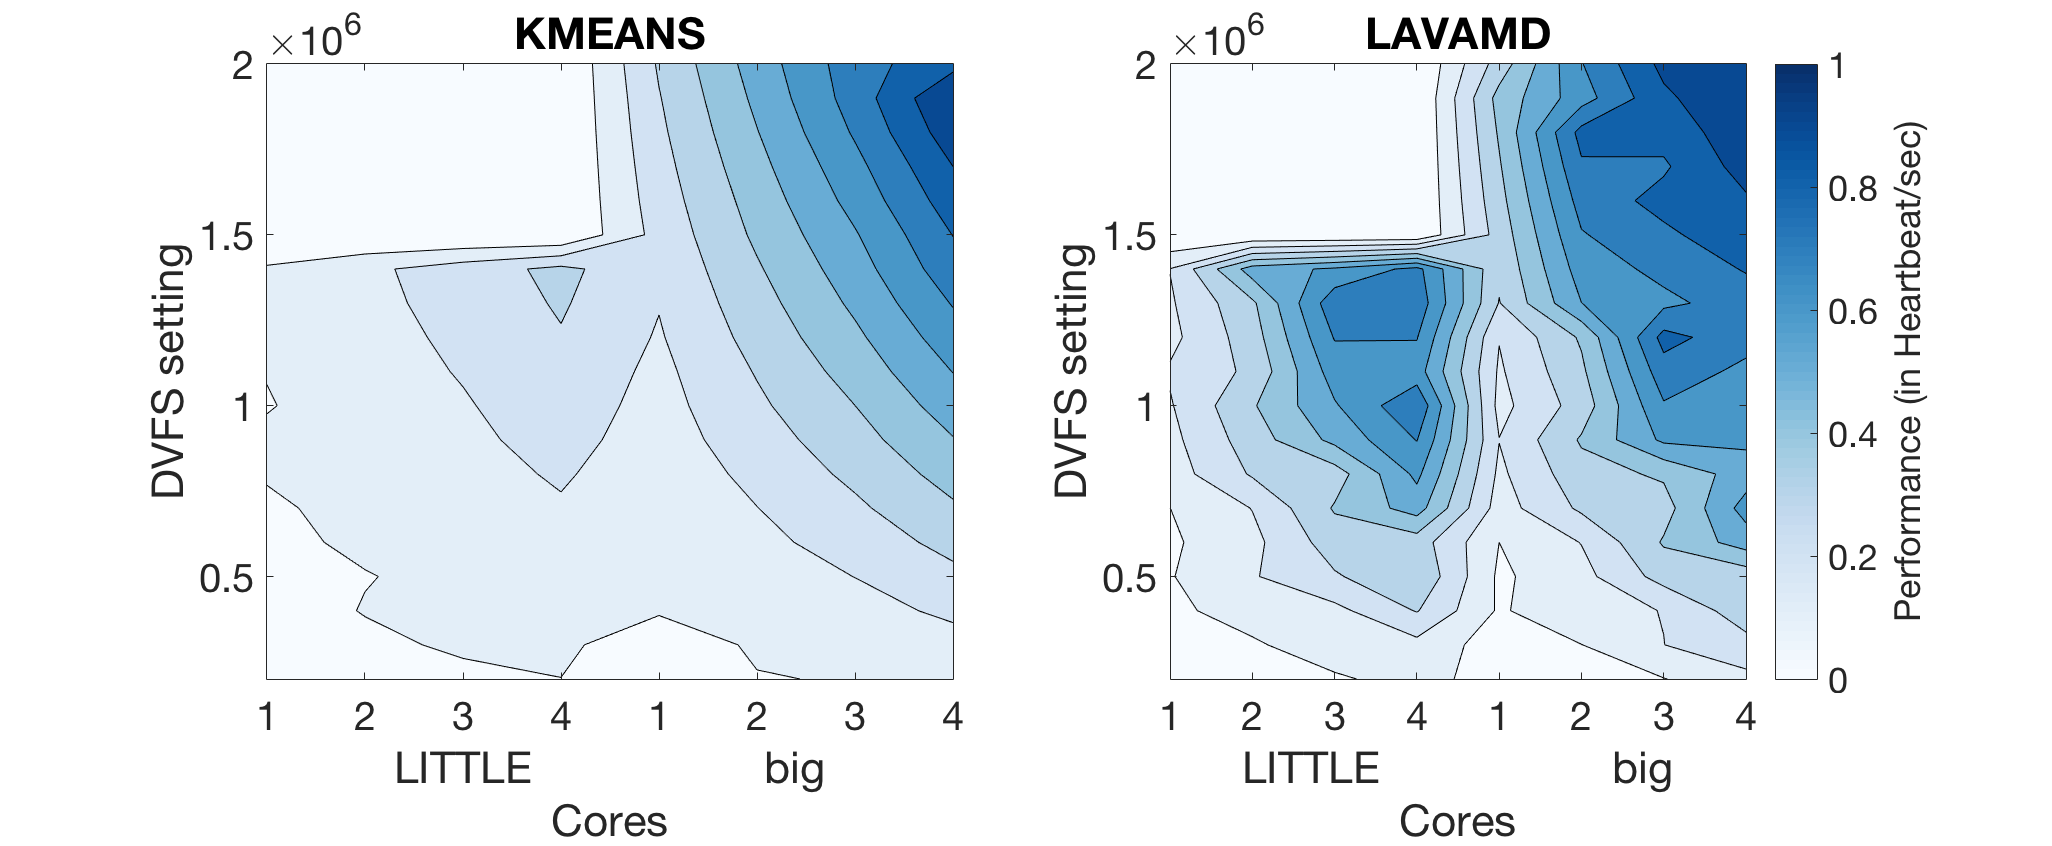
\includegraphics[width=\columnwidth]{figures/performance-contour2.png}
%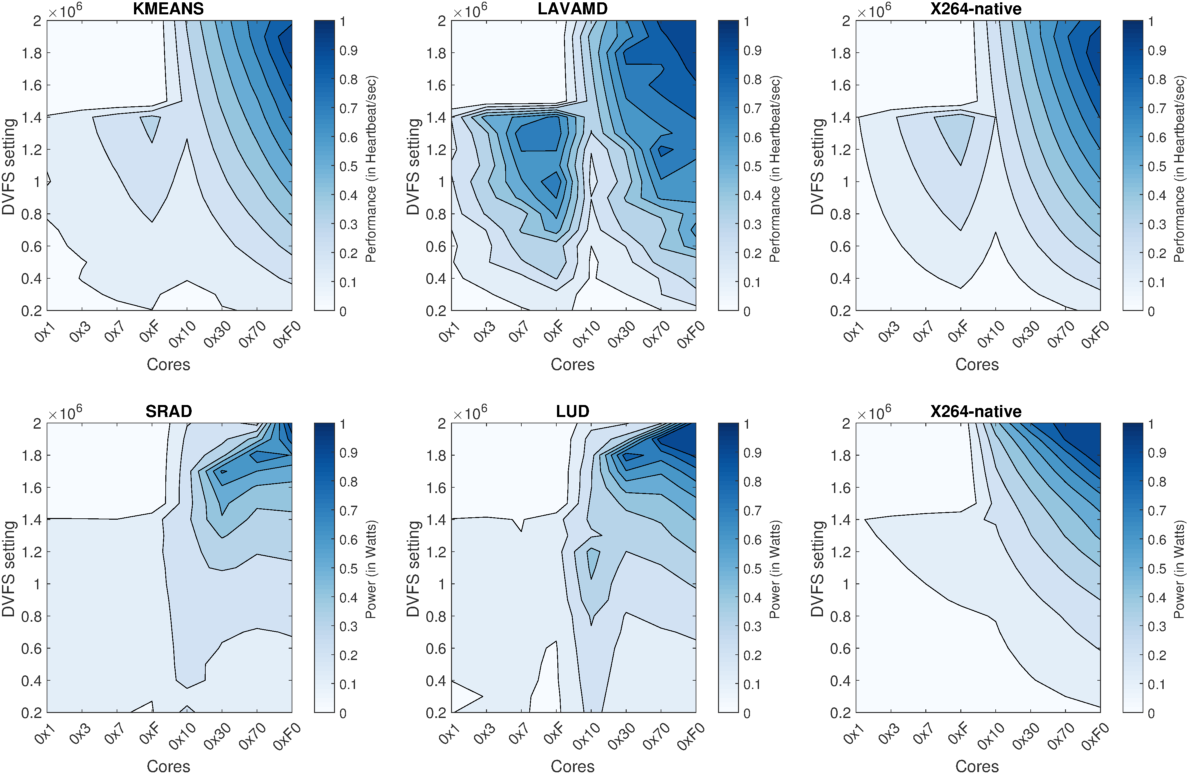
\includegraphics[scale=0.4]{figures/sample-contour3.png}
\caption{Contour plots showing performance as a function of core
  number, type, and speed.}
  \label{fig:contour}
\end{figure}

\begin{figure}[t]
  \begin{tikzpicture}
\begin{centering}

\definecolor{s1}{RGB}{228, 26, 28}
\definecolor{s2}{RGB}{55, 126, 184}
\definecolor{s3}{RGB}{77, 175, 74}
\definecolor{s4}{RGB}{152, 78, 163}
\definecolor{s5}{RGB}{255, 127, 0}

\begin{groupplot}[
    group style={
        group name=plots,
        group size=1 by 1,
        xlabels at=edge bottom,
        xticklabels at=edge bottom,
        vertical sep=5pt
    },
height=3.5cm,
width=0.95\columnwidth,
xmajorgrids,
ymajorgrids,
grid style={dashed},
xmin=0,
xmax=20,
yticklabel pos=left,
enlargelimits=false,
tick align = outside,
tick style={white},
xticklabel shift={-5pt},
yticklabel shift={-5pt},
ylabel shift={-2pt},
ylabel style={align=center},
unbounded coords=jump,
]

\nextgroupplot[ylabel={\footnotesize Performance \\ (Normalized)}, % Performance
%xtick={0,500,1000,1500,2000,2500,3000,3500,4000,4500},
ytick={0.0,0.5,1.0,1.5,2.0},
yticklabels={,0.5,1.0,1.5,2.0},
%xtick={0,30,60,120,160,200,240,280,320,480},
%xticklabels={,0,30,60,120,160,200,240,280,320,480},
yticklabel style={font=\footnotesize},
ymin=0,
ymax=1.5,
legend entries={,{$\mathsf{Learning}$},{$\mathsf{Control}$}},
legend style={draw=none,at={(0.5,1.4)},anchor=north,legend columns=4,line width=5pt},
]

\addplot[thick, dashed, black] coordinates {(10,0) (10,1.5)};
\addplot[thick, solid, color=s4] table[x index=0,y index=1,col sep=tab] {img/image_text/kmeans-example.txt};
\addplot[thick, solid, color=s5] table[x index=0,y index=2,col sep=tab] {img/image_text/kmeans-example.txt};
%\addplot[thick, dashed, black] coordinates {(130,0) (130, 2)};
\end{groupplot}
\end{centering}

\end{tikzpicture}

   \vskip -1em
  \caption{Performance Control for KMEANS}
  \label{fig:kmeans-example}
\end{figure}
}




